\documentclass[11pt, oneside]{article}
\usepackage[letterpaper, margin=2cm]{geometry}
\usepackage{MATH667}
\usepackage{booktabs}
\newcommand{\doubletilde}[1]{\tilde{\tilde{#1}}}

\begin{document}
\noindent \textbf{\Large{Caleb Logemann \\
MATH667 Hyperbolic Partial Differential Equations \\
Homework 7
}}

%\lstinputlisting[language=MATLAB]{H01_23.m}
\begin{enumerate}
  \item % #1
    Derive the following 3\textsuperscript{rd} order accuracy reconstruction
    for finite volume methods.
    \begin{align*}
      u_{j+1/2}^- &= -\frac{1}{6} \bar{u}_{j-1} + \frac{5}{6}\bar{u}_j + \frac{1}{3}\bar{u}_{j+1} \\
      u_{j+1/2}^+ &= \frac{1}{3} \bar{u}_{j} + \frac{5}{6}\bar{u}_{j+1} - \frac{1}{6}\bar{u}_{j+2}
    \end{align*}

    For this problem we would like to construct a quadractic polynomial $p(x)$
    such that $p$ matches the cell average on intervals $I_{j-1}$, $I_j$, and
    $I_{j+1}$.
    If we set
    $p(x) = a\p{x - x_{j+1/2}}^2 + b\p{x - x_{j-1/2}} + c$, then
    $p(x_{j-1/2}) = c$.
    We can then solve the following three equations for $c$.
    \begin{align*}
      \frac{1}{h} \dintt{x_{j-3/2}}{x_{j-1/2}}{p(x)}{x} &= \bar{u}_{j-1} \\
      \frac{1}{h} \dintt{x_{j-1/2}}{x_{j+1/2}}{p(x)}{x} &= \bar{u}_{j} \\
      \frac{1}{h} \dintt{x_{j+1/2}}{x_{j+3/2}}{p(x)}{x} &= \bar{u}_{j+1}
    \end{align*}
    These equation can be simplified as follows.
    \begin{align*}
      \frac{1}{3h}a \p{-h^3 + 8h^3} + \frac{1}{2h}b\p{h^2 - 4h^2} + c &= \bar{u}_{j-1} \\
      \frac{1}{3h}a \p{h^3} + \frac{1}{2h}b\p{-h^2} + c &= \bar{u}_{j} \\
      \frac{1}{3h}a \p{h^3} + \frac{1}{2h}b\p{h^2} + c &= \bar{u}_{j+1}
    \end{align*}
    Simplifying gives
    \begin{align*}
      \frac{7h^2}{3}a - \frac{3h}{2}b + c &= \bar{u}_{j-1} \\
      \frac{h^2}{3}a - \frac{h}{2}b + c &= \bar{u}_{j} \\
      \frac{h^2}{3}a + \frac{h}{2}b + c &= \bar{u}_{j+1}.
    \end{align*}
    Subtracting three times the second equation to the first equation and adding the last two equations gives
    \begin{align*}
      \frac{4h^2}{3}a - 2c &= \bar{u}_{j-1} - 3\bar{u}_j \\
      \frac{2h^2}{3}a + 2c &= \bar{u}_j + \bar{u}_{j+1}.
    \end{align*}
    Subtracting 2 times the second equation from the first gives
    \begin{align*}
      -6c &= \bar{u}_{j-1} - 5\bar{u}_j - 2\bar{u}_{j+1} \\
      c &= -\frac{1}{6}\bar{u}_{j-1} + \frac{5}{6}\bar{u}_j + \frac{1}{3}\bar{u}_{j+1}
    \end{align*}
    Thus we have for the first reconstruction that
    \[
      u^-_{j+1/2} = p(x_{j+1/2}) = c = -\frac{1}{6}\bar{u}_{j-1} + \frac{5}{6}\bar{u}_j + \frac{1}{3}\bar{u}_{j+1}
    \]

    We can now do this process again on the intervals $I_j$, $I_{j+1}$, and $I_{j+2}$.
    This only changes one of the equations.
    We now have
    \begin{align*}
      \frac{1}{h} \dintt{x_{j+3/2}}{x_{j+5/2}}{p(x)}{x} &= \bar{u}_{j+2} \\
      \frac{1}{3h}a \p{8h^3 - h^3} + \frac{1}{2h}b\p{4h^2 - h^2} + c &= \bar{u}_{j+2} \\
      \frac{7h^2}{3}a + \frac{3h}{2}b + c &= \bar{u}_{j+2}
    \end{align*}
    We must now solve the following three equations for $c$
    \begin{align*}
      \frac{h^2}{3}a - \frac{h}{2}b + c &= \bar{u}_{j} \\
      \frac{h^2}{3}a + \frac{h}{2}b + c &= \bar{u}_{j+1} \\
      \frac{7h^2}{3}a + \frac{3h}{2}b + c &= \bar{u}_{j+2}.
    \end{align*}
    Adding the first two equations and subtracting 3 times the second
    equation from the last equation gives
    \begin{align*}
      \frac{2h^2}{3}a + 2c &= \bar{u}_{j} + \bar{u}_{j+1} \\
      \frac{4h^2}{3}a + -2c &= \bar{u}_{j+2} - 3\bar{u}_{j+1}.
    \end{align*}
    Subtracting 2 times the first equation from the second equation gives
    \begin{align*}
      -6c &= -2\bar{u}_{j} - 5\bar{u}_{j+1} + \bar{u}_{j+2} \\
      c &= \frac{1}{3}\bar{u}_{j} + \frac{5}{6}\bar{u}_{j+1} - \frac{1}{6}\bar{u}_{j+2}
    \end{align*}
    This is the second reconstruction
    \[
      u^+_{j+1/2} = p(x_{j+1/2}) = c = \frac{1}{3}\bar{u}_{j} + \frac{5}{6}\bar{u}_{j+1} - \frac{1}{6}\bar{u}_{j+2} \\
    \]

  \item % #2 Done
    Consider to solve the 1D scalar conservation law.
    Show the 3rd order finite volume MUSCL scheme is TVD.
    Use Harten's Thereom.

    First I will write out explicitly what the 3rd order MUSCL scheme is.
    We started with the following two reconstructions.
    \begin{align*}
      u_{j+1/2}^- &= -\frac{1}{6} \bar{u}_{j-1} + \frac{5}{6}\bar{u}_j + \frac{1}{3}\bar{u}_{j+1} \\
      u_{j+1/2}^+ &= \frac{1}{3} \bar{u}_{j} + \frac{5}{6}\bar{u}_{j+1} - \frac{1}{6}\bar{u}_{j+2}
    \end{align*}
    Now define
    \begin{align*}
      \tilde{u}_j &= u_{j+1/2}^- - \bar{u}_j \\
      \doubletilde{u}_{j+1} &= u_{j+1/2}^+ + \bar{u}_{j+1}
    \end{align*}
    Now we will do a minmod limiter
    \begin{align*}
      \tilde{u}_j^{\text{mod}} = \minmod{\tilde{u}_j, \bar{u}_{j+1} - \bar{u}_j, \bar{u}_{j} - \bar{u}_{j-1}} \\
      \doubletilde{u}_{j+1}^{\text{mod}} = \minmod{\doubletilde{u}_{j+1}, \bar{u}_{j+2} - \bar{u}_{j+1}, \bar{u}_{j+1} - \bar{u}_{j}}
    \end{align*}
    Finally let
    \begin{align*}
      u_{j+1/2}^{-,\text{mod}} &= \bar{u}_j + \tilde{u}_j^{\text{mod}} \\
      u_{j+1/2}^{+,\text{mod}} &= \bar{u}_{j+1} - \doubletilde{u}_{j+1}^{\text{mod}}
    \end{align*}

    Now the full scheme is
    \[
      \bar{u}^{n+1}_j = \bar{u}^n_j - \frac{\Delta t}{\Delta x} \p{\hat{f}(u_{j+1/2}^{-,\text{mod}}, u_{j+1/2}^{+,\text{mod}}) - \hat{f}(u_{j-1/2}^{-,\text{mod}}, u_{j-1/2}^{+,\text{mod}})}
    \]

    In order to show that this scheme is TVD, we can rewrite this method as
    \[
      \bar{u}^{n+1}_j = \bar{u}^n_j - \frac{\Delta t}{\Delta x} \p{\hat{f}(u_{j+1/2}^{-,\text{mod}}, u_{j+1/2}^{+,\text{mod}}) - \hat{f}(u_{j+1/2}^{-,\text{mod}}, u_{j-1/2}^{+,\text{mod}}) +\hat{f}(u_{j+1/2}^{-,\text{mod}}, u_{j-1/2}^{+,\text{mod}}) - \hat{f}(u_{j-1/2}^{-,\text{mod}}, u_{j-1/2}^{+,\text{mod}})}
    \]
    Now we can write this method as
    \[
      \bar{u}^{n+1}_j = \bar{u}^n_j -  C_{j-1}\p{\bar{u}_j - \bar{u}_{j-1}} + D_j\p{\bar{u}_{j+1} - \bar{u}_j}
    \]
    where
    \begin{align*}
      C_{j-1} &= \frac{\Delta t}{\Delta x} \frac{\hat{f}(u_{j+1/2}^{-,\text{mod}}, u_{j-1/2}^{+,\text{mod}}) - \hat{f}(u_{j-1/2}^{-,\text{mod}}, u_{j-1/2}^{+,\text{mod}})}{\bar{u}_j - \bar{u}_{j-1}} \\
      D_{j} &= \frac{\Delta t}{\Delta x} \frac{\hat{f}(u_{j+1/2}^{-,\text{mod}}, u_{j-1/2}^{+,\text{mod}}) - \hat{f}(u_{j+1/2}^{-,\text{mod}}, u_{j+1/2}^{+,\text{mod}})}{\bar{u}_{j+1} - \bar{u}_{j}}
    \end{align*}

    Now Harten's Theorem states that this method is TVD if $C_{j-1} \ge 0$,
    $D_j \ge 0$, and $C_j + D_j \le 1$ for all $j$.

    First consider $C_{j-1}$
    \begin{align*}
      C_{j-1} &= \frac{\Delta t}{\Delta x} \frac{\hat{f}(u_{j+1/2}^{-,\text{mod}}, u_{j-1/2}^{+,\text{mod}}) - \hat{f}(u_{j-1/2}^{-,\text{mod}}, u_{j-1/2}^{+,\text{mod}})}{\bar{u}_j - \bar{u}_{j-1}} \\
      &= \frac{\Delta t}{\Delta x} \frac{\hat{f}(\bar{u}_j + \tilde{u}_j^{\text{mod}}, u_{j-1/2}^{+,\text{mod}}) - \hat{f}(\bar{u}_{j-1} + \tilde{u}_{j-1}^{\text{mod}}, u_{j-1/2}^{+,\text{mod}})}{\bar{u}_j - \bar{u}_{j-1}} \\
      &= \frac{\Delta t}{\Delta x} \hat{f}_1(\xi, u_{j-1/2}^{+,\text{mod}})\frac{\bar{u}_j + \tilde{u}_j^{\text{mod}} - \bar{u}_{j-1} - \tilde{u}_{j-1}^{\text{mod}}}{\bar{u}_j - \bar{u}_{j-1}} \\
      &= \frac{\Delta t}{\Delta x} \hat{f}_1(\xi, u_{j-1/2}^{+,\text{mod}})\p{1 + \frac{\tilde{u}_j^{\text{mod}}}{\bar{u}_j - \bar{u}_{j-1}} - \frac{\tilde{u}_{j-1}^{\text{mod}}}{\bar{u}_j - \bar{u}_{j-1}}}
      \intertext{Now since $\frac{\Delta t}{\Delta x} > 0$ and $\hat{f}_1(\xi, u_{j-1/2}^{+,\text{mod}}) > 0$ by monotonicity}
      C_{j-1} &\ge 1 + \frac{\tilde{u}_j^{\text{mod}}}{\bar{u}_j - \bar{u}_{j-1}} - \frac{\tilde{u}_{j-1}^{\text{mod}}}{\bar{u}_j - \bar{u}_{j-1}}
      \intertext{Also $0 \le \tilde{u}_j^{\text{mod}} \le \bar{u}_j - \bar{u}_{j-1}$ and $0 \le \tilde{u}_{j-1}^{\text{mod}} \le\bar{u}_j - \bar{u}_{j-1}$, so}
      C_{j-1} &\ge 1 + 0 - 1 = 0
    \end{align*}
    This shows that $C_{j-1} \ge 0$ for all $j$, so now consider $D_j$.
    \begin{align*}
      D_{j} &= \frac{\Delta t}{\Delta x} \frac{\hat{f}(u_{j+1/2}^{-,\text{mod}}, u_{j-1/2}^{+,\text{mod}}) - \hat{f}(u_{j+1/2}^{-,\text{mod}}, u_{j+1/2}^{+,\text{mod}})}{\bar{u}_{j+1} - \bar{u}_{j}} \\
      &= \frac{\Delta t}{\Delta x}\frac{\hat{f}(u_{j+1/2}^{-,\text{mod}}, \bar{u}_{j} - \doubletilde{u}_j^{\text{mod}}) - \hat{f}(u_{j+1/2}^{-,\text{mod}}, \bar{u}_{j+1} - \doubletilde{u}_{j+1}^{\text{mod}})}{\bar{u}_{j+1} - \bar{u}_{j}} \\
      &= \frac{\Delta t}{\Delta x}\hat{f}_2(u_{j+1/2}^{-,\text{mod}}, \xi)\frac{\bar{u}_{j} - \doubletilde{u}_j^{\text{mod}} - \bar{u}_{j+1} + \doubletilde{u}_{j+1}^{\text{mod}}}{\bar{u}_{j+1} - \bar{u}_{j}} \\
      &= \frac{\Delta t}{\Delta x}\hat{f}_2(u_{j+1/2}^{-,\text{mod}}, \xi)\p{-1 - \frac{\doubletilde{u}_j^{\text{mod}}}{\bar{u}_{j+1} - \bar{u}_{j}} + \frac{\doubletilde{u}_{j+1}^{\text{mod}}}{\bar{u}_{j+1} - \bar{u}_{j}}}
      \intertext{Now since $\frac{\Delta t}{\Delta x} \ge 0$, $\hat{f}_2(u_{j+1/2}^{-,\text{mod}}, \xi) \le 0$ by monotonicity, $0 \le \doubletilde{u}_j^{\text{mod}} \le \bar{u}_{j+1} - \bar{u}_j$, and $0 \le \doubletilde{u}_{j+1}^{\text{mod}} \le \bar{u}_{j+1} - \bar{u}_j$, this implies that}
      0 &\ge \p{-1 - \frac{\doubletilde{u}_j^{\text{mod}}}{\bar{u}_{j+1} - \bar{u}_{j}} + \frac{\doubletilde{u}_{j+1}^{\text{mod}}}{\bar{u}_{j+1} - \bar{u}_{j}}} \\
      D_{j} &\ge 0
    \end{align*}
    Lastly consider $C_j + D_j$,
    \begin{align*}
      C_j + D_j &= \frac{\Delta t}{\Delta x} \frac{\hat{f}(u_{j+3/2}^{-,\text{mod}}, u_{j+1/2}^{+,\text{mod}}) - \hat{f}(u_{j+1/2}^{-,\text{mod}}, u_{j+1/2}^{+,\text{mod}})}{\bar{u}_{j+1} - \bar{u}_{j}} + \frac{\Delta t}{\Delta x} \frac{\hat{f}(u_{j+1/2}^{-,\text{mod}}, u_{j-1/2}^{+,\text{mod}}) - \hat{f}(u_{j+1/2}^{-,\text{mod}}, u_{j+1/2}^{+,\text{mod}})}{\bar{u}_{j+1} - \bar{u}_{j}} \\
      &= \frac{\Delta t}{\Delta x} \p{\hat{f}_1(\xi, u_{j+1/2}^{+,\text{mod}})\p{1 + \frac{\tilde{u}_{j+1}^{\text{mod}}}{\bar{u}_{j+1} - \bar{u}_{j}} - \frac{\tilde{u}_{j}^{\text{mod}}}{\bar{u}_{j+1} - \bar{u}_{j}}} + \hat{f}_2(u_{j+1/2}^{-,\text{mod}}, \xi)\p{-1 - \frac{\doubletilde{u}_j^{\text{mod}}}{\bar{u}_{j+1} - \bar{u}_{j}} + \frac{\doubletilde{u}_{j+1}^{\text{mod}}}{\bar{u}_{j+1} - \bar{u}_{j}}}}
      \intertext{Let $\nu = \max{\abs{\hat{f}_1(\xi, u_{j+1/2}^{+,\text{mod}})}, \abs{\hat{f}_2(u_{j+1/2}^{-,\text{mod}}, \xi)}}$, then}
      C_j + D_j &\le \frac{\nu \Delta t}{\Delta x} \p{1 + \frac{\tilde{u}_{j+1}^{\text{mod}}}{\bar{u}_{j+1} - \bar{u}_{j}} - \frac{\tilde{u}_{j}^{\text{mod}}}{\bar{u}_{j+1} - \bar{u}_{j}} + 1 + \frac{\doubletilde{u}_j^{\text{mod}}}{\bar{u}_{j+1} - \bar{u}_{j}} - \frac{\doubletilde{u}_{j+1}^{\text{mod}}}{\bar{u}_{j+1} - \bar{u}_{j}}} \\
      C_j + D_j &\le \frac{4 \nu \Delta t}{\Delta x}
      \intertext{If $\Delta t$ is chosen such that $0 < \Delta t \le \frac{\Delta x}{4 \nu}$, then}
      C_j + D_j & \le 1
    \end{align*}
    This show that the third order MUSCL scheme is TVD, by Harten's Theorem.

  \item % #3 Done
    Solve two-phase flow nonconver Buckley-Leverett equation with
    3\textsuperscript{rd} order finite volume MUSCL scheme.
    \[
      u_t + \p{\frac{2u^2}{2u^2 + (1 - u)^2}}_x = 0
    \]
    with initial conditions
    \[
      u(x, 0) =
      \begin{cases}
        1 & x \le 0 \\
        0 & x > 0
      \end{cases}
    \]
    The solution consists of a rarefaction wave connecting with a shock, ref
    to Figure 4.7 on page 49.
    Simulate the evolution of the solution to $T = 1.0$ with total mesh
    $N = 100$.
    Output the simulate with one symbol per cell on the figure.
    Use exact solutions at the boundary (ghost cells) as the given boundary
    conditions.

    The following is my third order MUSCL scheme
    \lstinputlisting[language=MATLAB]{muscl3.m}
    The following script now uses this function to solve the Buckley-Leverett equation.
    \lstinputlisting[language=MATLAB]{H07.m}
    The following image is produced.
    \begin{center}
      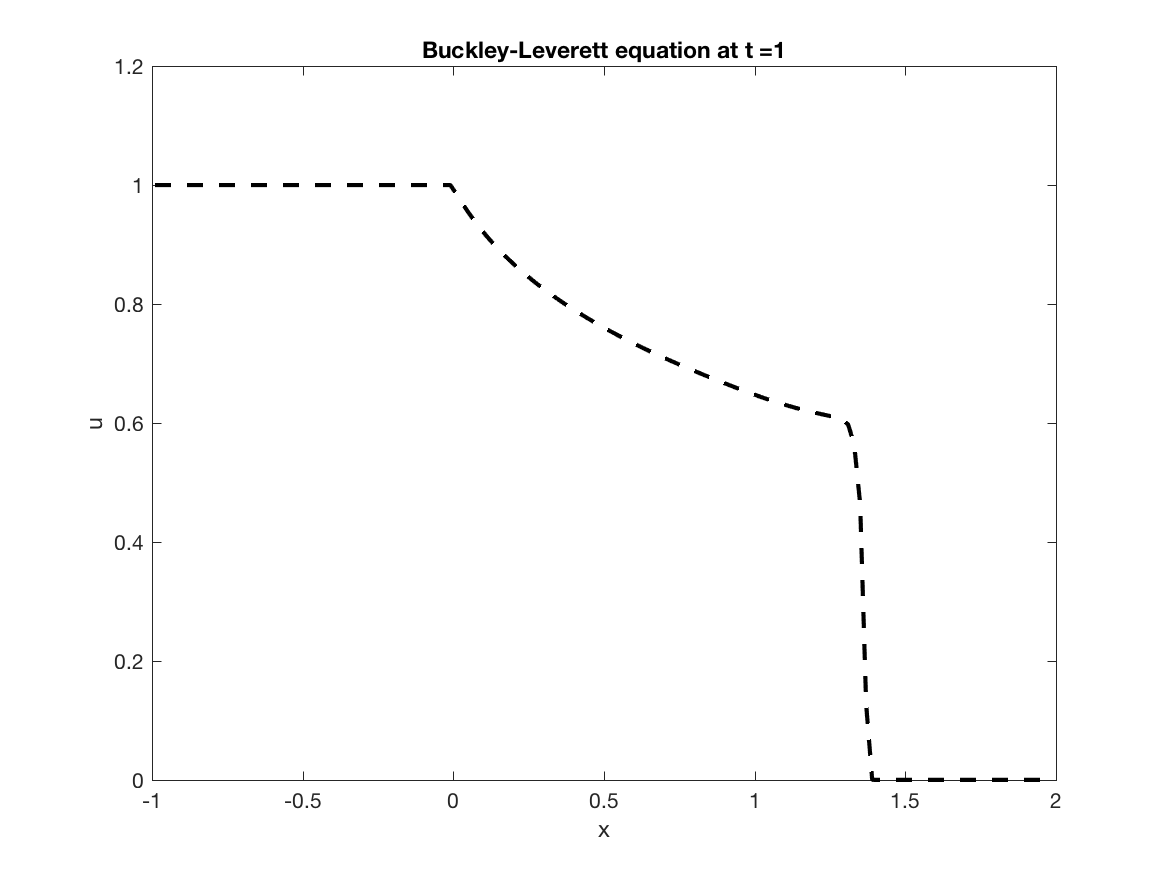
\includegraphics[scale=0.8]{Figures/07_01.png}
    \end{center}
\end{enumerate}
\end{document}
